\textbf{Example}

Let $M=4$, $N=4$, and $A=[1,2,1,3]$. The grader calls \texttt{create\_circuit(4, [1, 2, 1,
3])}.


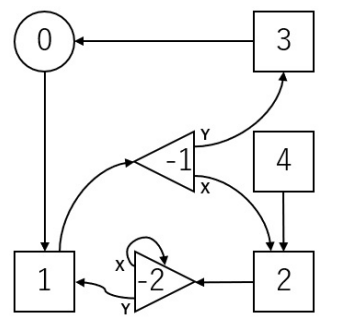
\includegraphics{4.png}

The above figure shows a circuit, which is described by a call \texttt{answer([1, -1, -2, 0,
2], [2, -2], [3, 1])}. The numbers in the figure are the serial numbers of the
devices.

Two switches are used. Thus $S=2$.

Initially, the states of the switches $-1$ and $-2$ are both `X'.

The ball travels as follows:

$0\rightarrow 1 \rightarrow -1 \stackrel{X}\rightarrow 2 \rightarrow -2 \stackrel{X}\rightarrow -2 \stackrel{Y}\rightarrow 1 \rightarrow -1 \stackrel{Y}\rightarrow 3 \rightarrow 0$ 

\begin{itemize}
    \item When the ball first enters the switch $-1$, its state is `X'. Hence, the ball travels to
the trigger $2$. Then the state of the switch $-1$ is changed to `Y'.
\item When the ball enters the switch $-1$ for the second time, its state is `Y'. Hence, the ball travels to the trigger $3$. Then the state of the switch $-1$ is changed to `X'.
\end{itemize}

The ball first returns to the origin, having entered the triggers $1,2,1,3$. The states of
the switches $-1$ and $-2$ are both `X'. The value of $P$ is $4$. Therefore, this circuit
satisfies the conditions.

The file sample-01-in.txt in the zipped attachment package corresponds to this
example. Other sample inputs are also available in the package.